\documentclass[../../thesis.tex]{subfiles}

\graphicspath{{./img/}}

\begin{document}

In the previous section, we identify the hidden patterns in our temporal network sample. We continue our work by investigating the possibility of modeling the Bitcoin transactions temporal network. In this section, we propose an analytical model that aims to identify statistical regularities of the distribution of the motifs counts (see sec[motif]) from our Bitcoin transactions temporal network sample (see Section~\ref{sec:bitcoin_as_a_graph}). We achieve this by modifying the activity driven model proposed by \cite{perra2012activity}. 



\section{Activity driven modeling of time varying networks}
\label{sec:activity_driven_model}

The vast majority of recent modeling approaches are connectivity driven \cite{1newman2010networks,2barrat2008dynamical,3albert2002statistical,4boccaletti2006complex,5bollobas2013modern,6vespignani2012modelling,8molloy1995critical,9holland1981exponential,10frank1986markov,11wasserman1996logit,12barabasi1999mean,13barabasi1999emergence,14dorogovtsev2000structure,15dorogovtsev2013evolution,16fortunato2006scale,17boguna2003class}, where the network’s topology is at the core of the model’s algorithmic definition. Connectivity-driven network models are well-suited for capturing the essential features of systems such as the Internet, where connections among nodes are long-lived elements \cite{18pastor2007evolution,19albert1999internet}. However, in many cases, the interactions between the elements of the system are rapidly changing and are characterized by processes whose timing and duration are defined on a very short time scale \cite{temporalNetworks,21ghoshal2006attractiveness}. Connectivity driven models necessarily provide a time-aggregated representation that may fail to describe the instantaneous and fluctuating dynamics of many networks, including the network which we are dealing with. The motivation of using an activity driven model as the base of our model is defined by the capability of the model proposed by \cite{perra2012activity} to encode the instantaneous time description of the network dynamics.  The work of \cite{perra2012activity} introduces a framework which can analytically describe highly dynamical networks. Their models intend to capture the process of accumulating connections over time and the resulting degree distribution and other topological properties merely represent a time-integrated perspective of the system. They conclude that the dynamics of the network can be encoded by the activity potential distribution function from which it is possible to derive the appropriate interaction rate among nodes. Proposing a process model for the generation of random dynamic networks can be used as a general base model for rapidly evolving networks.


\subsection{The Activity Potential}
\label{sec:activity_driven_model_activity_potential}


The activity potential characterizes the individual activity of every agent, in our case, the number of Bitcoin transactions made. Activity potential $x_{i}$ of the agent $i$ is the number of interactions that he performs in a given particular time window of length $\Delta t$, divided by the total number of connections made by all agents during that same time window. It estimates the probability that the agent $i$ was involved in any given interaction in the system.  Interaction dynamics of the system is defined statistically by the probability distribution $F(x)$ that a randomly chosen agent $i$ has an activity potential $x$.


\subsection{General Activity driven network model}
\label{sec:activity_driven_model_network}

We describe the general activity driven model for time-varying networks proposed by \cite{perra2012activity}. The general model uses the activity distribution to drive the formation of a dynamic system.

For each node (agent) $i$ we assign an activity firing rate $a_{i}=\eta x_{i}$, where $x_{i}$ are bound by the interval  $\mathcal{E} \leq x_{i} \leq 1$. The activity firing rate is the probability per unit time to create new edges with other nodes, which is assigned according to a given probability distribution $F(x)$ that may be chosen arbitrarily or given by empirical data. $\eta$ is a rescaling factor. The work of \cite{perra2012activity} proposes a simple generative process according to the following rules:
\begin{enumerate}
  \item{At each discrete time step $t$ the network $G_{t}$ starts with $N$ disconnected nodes.}
  \item{With probability $a_{i}\Delta t$ each node $i$ becomes active and generates $m$ links that are connected to $m$ other randomly selected nodes. Non-active nodes can still receive connections from other active nodes.}
  \item{At the next time step $t+\Delta t$, all the edges in the network $G_{t}$ are deleted. }
\end{enumerate}

Figure~\ref{fig:activity_driven_model} illustrates the process of the general model from \cite{perra2012activity}. Considering an example of 13 nodes and $m=3$. We plot the  resulting networks for three different time steps. The red nodes represent the active nodes and the grey nodes represent the inactive nodes. The dashed lines represent the past connections. From this definition we can see that all interactions have a constant duration $T_{i}=\Delta t$. The agents do not have a memory of the previous time steps. The full dynamics of the network and its resulting structure is therefore entirely encoded in the activity potential distribution function $F(x)$. This function allows the definition of a simple dynamical process based on the nodes’ activity rate, providing a time dependent description of the network’s connectivity pattern.

\begin{figure}
\centering
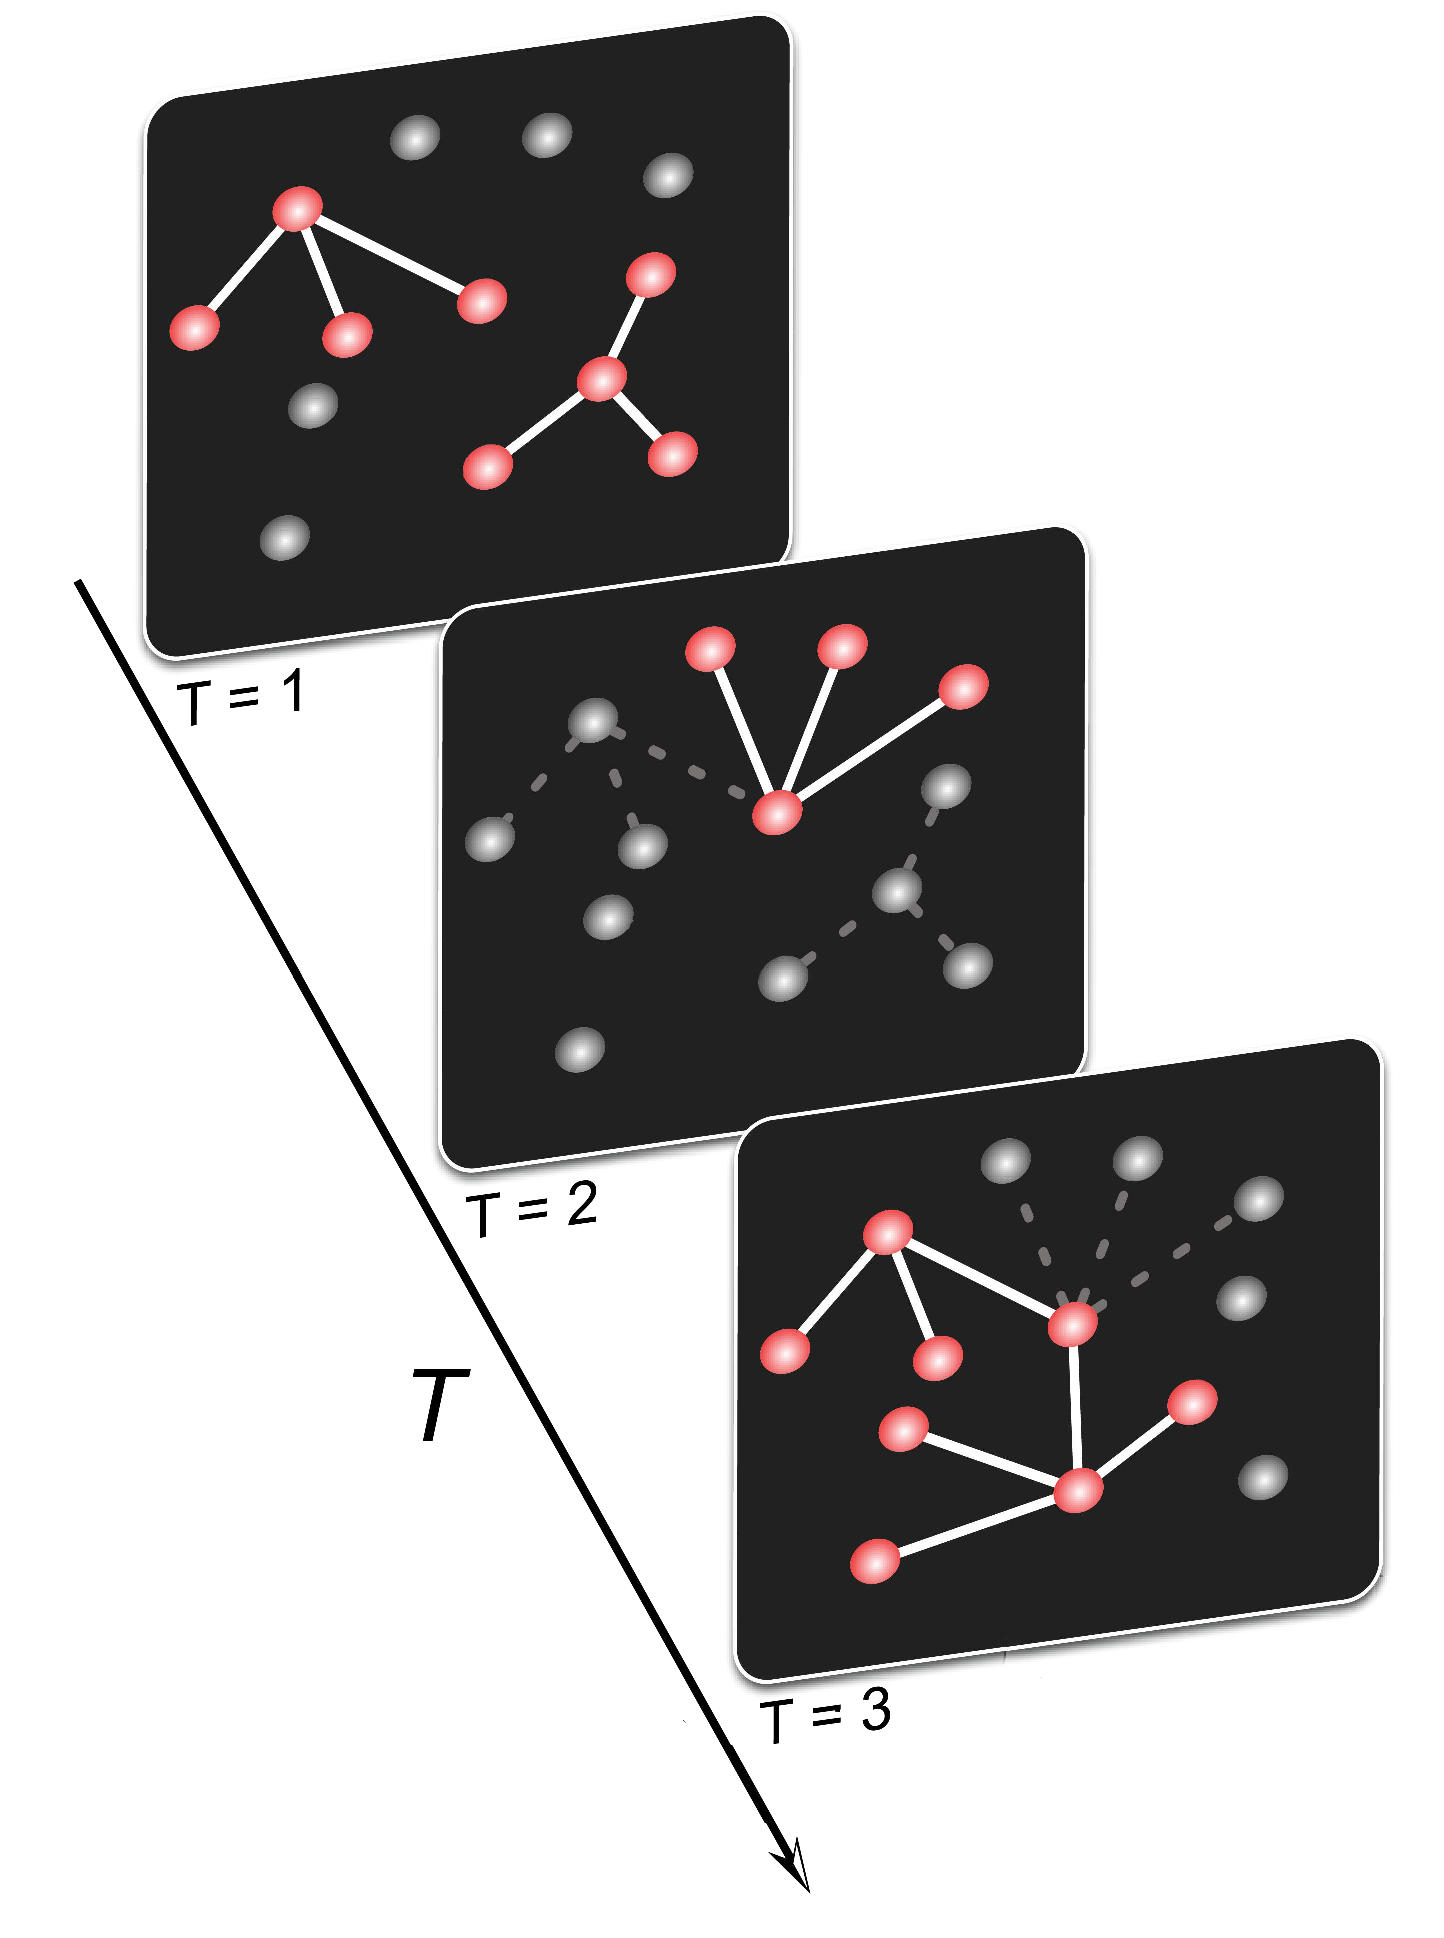
\includegraphics[width=0.45\textwidth]{content/modelling/img/activity_driven_model}
\caption{Illustration of the general model process from \ref{sec:activity_driven_model_network}. Considering 13 nodes and $m=3$, we visualize the resulting networks for three different time steps. The red nodes represent the active nodes and the grey nodes represent the not active nodes. The dash lines represent the past connections.}
\label{fig:activity_driven_model}
\end{figure}

\subsection{Applying the General Activity Driven Model to simulate the Bitcoin transactions temporal network}
\label{sec:activity_driven_model_network}

Despite its simplicity, the model stresses that the actors’ activity rate plays a significant role in the understanding of dynamical networks. With this feature, we see the potential of this model for simulating the Bitcoin transactions temporal network where, only the agents, the ones who make transactions, define the network. We now investigate how suitable this general model is for capturing the dynamics of our network over our data sample.

In Section~\ref{sec:motifs_bitcoin}, we selected three sample days to be our golden models: \textit{Day A) May 4 2017; Day B) June 16 2017; Day C) August 1 2017;} Where, considering only the 6 most relevant motifs: $M_{1,6}$,$M_{6,6}$, $M_{1,1}$, $M_{2,5}$, $M_{1,5}$ and $M_{2,6}$. Day \textit{A)} has a lower motifs counts, day \textit{B)} has a higher motifs counts and day \textit{C)} has high volatility, marked by the Bitcoin break of consensus [\href{https://www.cnbc.com/2017/07/31/blockchain-fork-will-create-new-digital-crypto-currency-bitcoin-cash.html}{1}, \href{https://www.theverge.com/2017/8/1/16075276/bitcoin-cash-hard-fork-coinbase}{2}, \href{https://motherboard.vice.com/en_us/article/9kwepa/bitcoin-has-forked}{3}, \href{https://techcrunch.com/2017/08/02/wtf-is-bitcoin-cash-and-is-it-worth-anything/}{4}, \href{http://money.cnn.com/2017/08/01/technology/business/bitcoin-cash-new-currency/index.html}{5}]. Our goal now is to use the general model described in \ref{sec:activity_driven_model_network} to simulate one day of Bitcoin transactions. We chose this model because we are interested in discovering how the edges are made and not how the network grows. Thus, the model proposed by \cite{perra2012activity} provides for us a ground zero model for generating random edges. Afterwards, we run the algorithm from \ref{sec:motifs_couting} to count the temporal motifs with $\delta = 1$ hour as the parameter. We count the motifs on the simulated temporal network output and on the selected samples days. Then, we normalize the counts to compare the distribution of the motifs counts. We compare them using the root-mean-square error function: 
\begin{equation} 
\label{eq1}
\begin{split}
\operatorname{RMSE}= \sqrt{\frac{1}{n}\sum_{j=1}^{n}{(P_{i}-O_{i})}^{2}}
\end{split}
\end{equation}
An error close to one means the simulation did not capture the dynamics. We run our first experiment of with no modifications on the general model of Section~\ref{sec:activity_driven_model_network}, moreover with the initial parameters: Number of nodes $N=100$; $\Delta$t$=1$, Number of Connections $m=10$, Activity Distribution Function $F(x)=$ Pareto Distribution with $\alpha=2$, 5000 steps and Temporal Motif $\delta=$ 1 hour. 

Our first simulation comparing to day A) was able to achieve error $E=0.583254$. Comparing to day B) $E=0.389751$ and comparing to day C) $E=0.642245$. Although we achieved a good distribution, the motifs $M_{2,4}$(triangle), $M_{3,5}$(triangle), $M_{5,1}$(cycle-2-nodes), $M_{5,2}$(cycle-2-nodes), $M_{6,2}$(cycle-2-nodes) were not generated by the simulations. However, those motifs are quite irrelevant in the real data. Figure \ref{fig:all_motifs_golden_vs_simulation_activitydriven} helps to visualize the distribution of the motifs between the selected days and the simulation.

\begin{figure}[H]
\centering
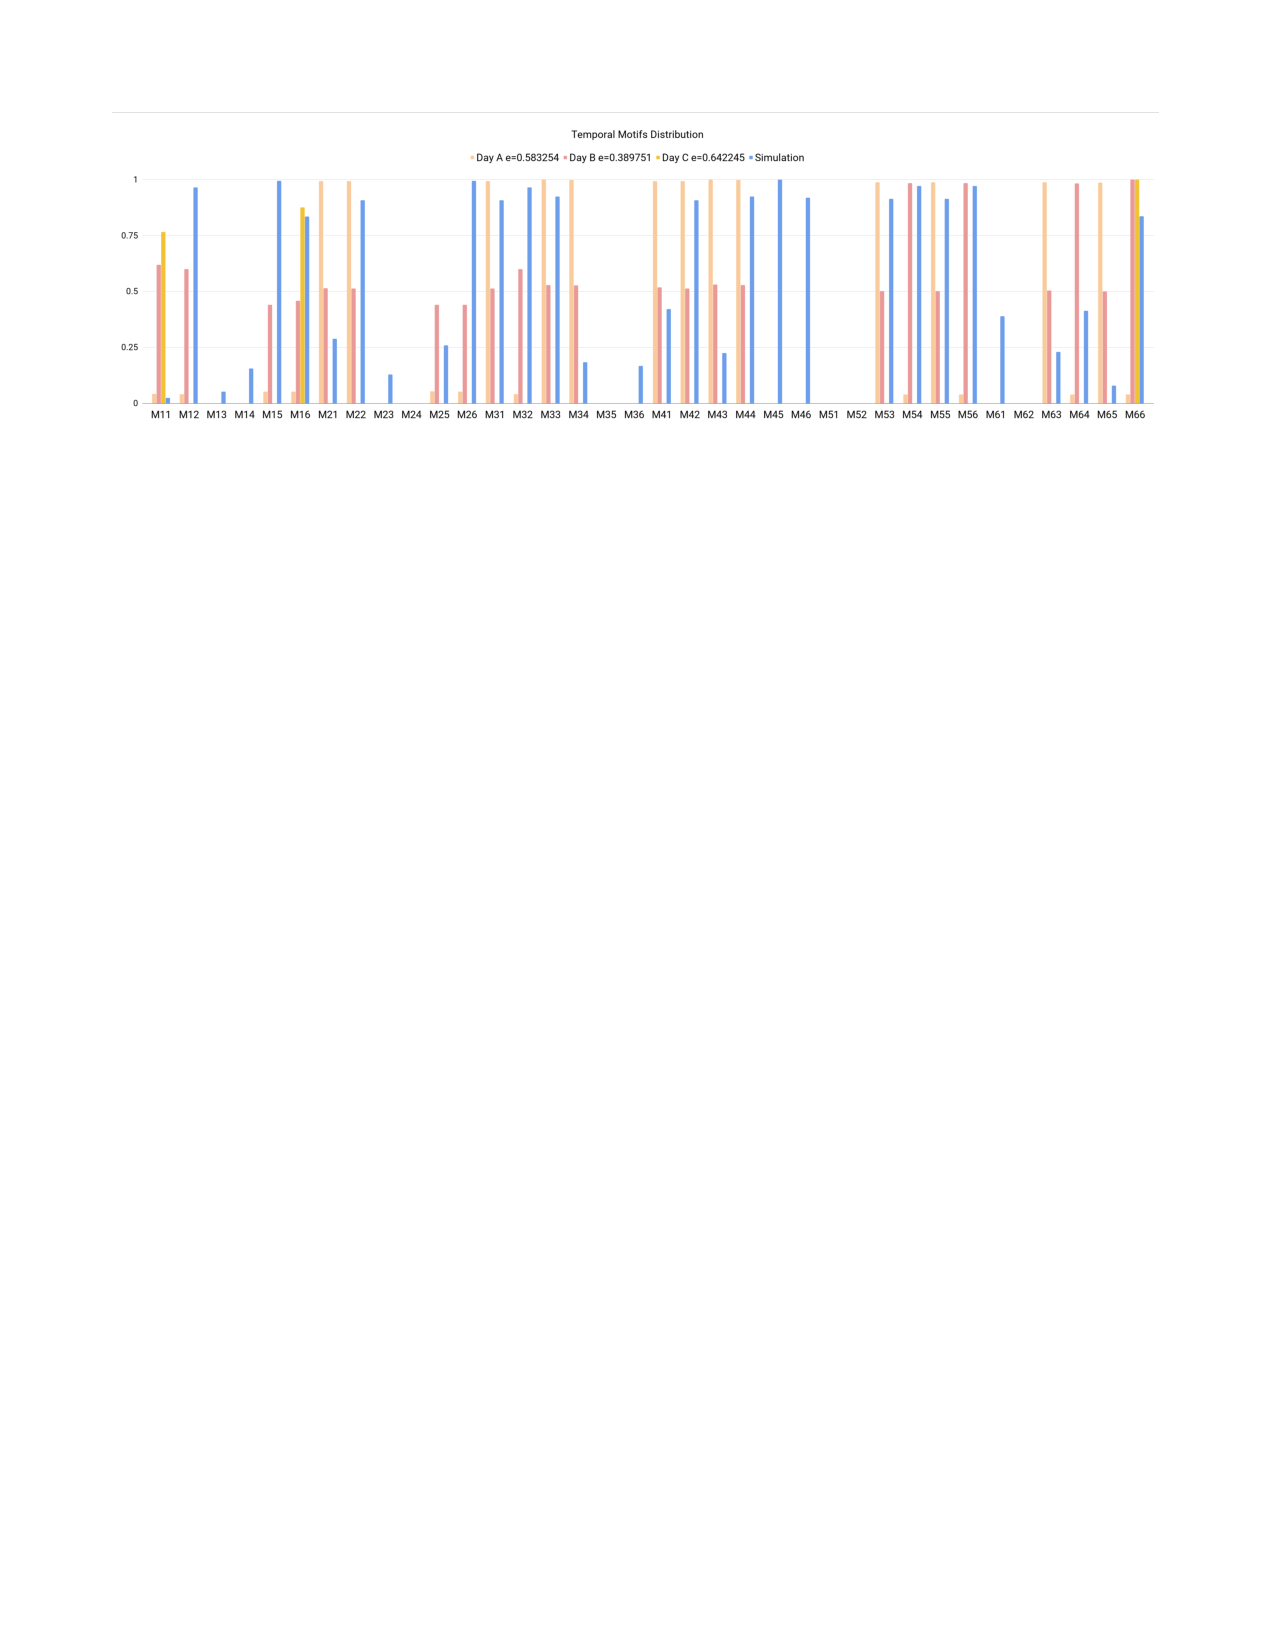
\includegraphics[width=\textwidth]{content/modelling/img/all_motifs_golden_activity_vs_simulation_norm_activitydriven151563604500.pdf}
\caption{Distribution of the motifs normalized between the selected days and the activity driven simulation, using the parameters: Number of nodes $N=100$; $\Delta$t$=1$, Number of Connections $m=10$, Activity Distribution as Pareto with $\alpha=2$, 5000 steps and Temporal Motif $\delta=$ 1 hour. Comparing the simulation to day A) the simulation was able to achieve error $E=0.583254$. Comparing to day B) $E=0.389751$ and comparing to day C) $E=0.642245$. Additionally, the motifs $M_{2,4}$(triangle), $M_{3,5}$(triangle), $M_{5,1}$(cycle-2-nodes), $M_{5,2}$(cycle-2-nodes), $M_{6,2}$(cycle-2-nodes) were never generated by the simulation.}
\label{fig:all_motifs_golden_vs_simulation_activitydriven}
\end{figure}

Several attempts with different parameters were made to get better results but none was relevant. We know that the General Model is a \textit{Markovian} model, where the future states depend only on the current state. Although, in order to model the Bitcoin dynamics, we intuitively assume: agents that have traded in the past are more likely to trade again among them. Thus, this assumption adds memory to our agents. Additionally, memory feature is not covered by the general model of subsection \ref{sec:activity_driven_model_network}. This lack of memory encourages us to modify the general activity driven model by allowing memory on the agents in order to look for better results.


\end{document}

         